\documentclass{article}

\usepackage{fancyhdr}
\usepackage{extramarks}
\usepackage{amsmath}
\usepackage{amsthm}
\usepackage{amsfonts}
\usepackage{tikz}
\usepackage[plain]{algorithm}
\usepackage{algpseudocode}
\usepackage[utf8]{inputenc}
\usepackage[T1]{fontenc}
\usepackage{natbib}
\usepackage{listings}
\usepackage{hyperref}

\usetikzlibrary{automata,positioning}

%
% Basic Document Settings
%

\topmargin=-0.45in
\evensidemargin=0in
\oddsidemargin=0in
\textwidth=6.5in
\textheight=9.0in
\headsep=0.25in

\linespread{1.1}

\pagestyle{fancy}
%\lhead{\hmwkAuthorName}
%\chead{\hmwkClass\ (\hmwkClassInstructor\ \hmwkClassTime): \hmwkTitle}
\lhead{\hmwkClass: \hmwkTitle}
\rhead{\hmwkAuthorName}
\lfoot{\lastxmark}
\cfoot{\thepage}

\renewcommand\headrulewidth{0.4pt}
\renewcommand\footrulewidth{0.4pt}

\setlength\parindent{0pt}
\setlength{\parskip}{1em}

%
% Create Problem Sections
%

\newcommand{\enterProblemHeader}[1]{
    \nobreak\extramarks{}{Problem \arabic{#1} continued on next page\ldots}\nobreak{}
    \nobreak\extramarks{Problem \arabic{#1} (continued)}{Problem \arabic{#1} continued on next page\ldots}\nobreak{}
}

\newcommand{\exitProblemHeader}[1]{
    \nobreak\extramarks{Problem \arabic{#1} (continued)}{Problem \arabic{#1} continued on next page\ldots}\nobreak{}
    \stepcounter{#1}
    \nobreak\extramarks{Problem \arabic{#1}}{}\nobreak{}
}

\setcounter{secnumdepth}{0}
\newcounter{partCounter}
\newcounter{homeworkProblemCounter}
\setcounter{homeworkProblemCounter}{1}
%\nobreak\extramarks{Problem \arabic{homeworkProblemCounter}}{}\nobreak{}

%
% Homework Problem Environment
%
% This environment takes an optional argument. When given, it will adjust the
% problem counter. This is useful for when the problems given for your
% assignment aren't sequential. See the last 3 problems of this template for an
% example.
%
\newenvironment{homeworkProblem}[1][-1]{
    \ifnum#1>0
        \setcounter{homeworkProblemCounter}{#1}
    \fi
    \section{Problem \arabic{homeworkProblemCounter}}
    \setcounter{partCounter}{1}
    \enterProblemHeader{homeworkProblemCounter}
}{
    \exitProblemHeader{homeworkProblemCounter}
}

%
% Homework Details
%   - Title
%   - Due date
%   - Class
%   - Section/Time
%   - Instructor
%   - Author
%

\newcommand{\hmwkTitle}{Exercices}
\newcommand{\hmwkDueDate}{5 février, 2017}
\newcommand{\hmwkClass}{MTH8408}
\newcommand{\hmwkClassTime}{}
\newcommand{\hmwkClassInstructor}{Professeur Dominique Orban}
\newcommand{\hmwkAuthorName}{André Phu-Van Nguyen}
\renewcommand{\refname}{Références}

%
% Title Page
%

\title{
    \vspace{2in}
    \textmd{\textbf{\hmwkClass:\ \hmwkTitle}}\\
%    \normalsize\vspace{0.1in}\small{Remis\ pour\ le\ \hmwkDueDate\ }\\
%    \vspace{0.1in}\large{\textit{\hmwkClassInstructor\ \hmwkClassTime}}
    \vspace{4in}
}

\author{\textbf{\hmwkAuthorName}}
\date{}

\renewcommand{\part}[1]{\textbf{\large Part \Alph{partCounter}}\stepcounter{partCounter}\\}

%
% Various Helper Commands
%

% Useful for algorithms
\newcommand{\alg}[1]{\textsc{\bfseries \footnotesize #1}}

% For derivatives
\newcommand{\deriv}[1]{\frac{\mathrm{d}}{\mathrm{d}x} (#1)}

% For partial derivatives
\newcommand{\pderiv}[2]{\frac{\partial}{\partial #1} (#2)}

% Integral dx
\newcommand{\dx}{\mathrm{d}x}

% Alias for the Solution section header
\newcommand{\solution}{\textbf{\large Solution}}
\newcommand{\norm}[1]{\left\lVert#1\right\rVert}

% Probability commands: Expectation, Variance, Covariance, Bias
\newcommand{\E}{\mathrm{E}}
\newcommand{\Var}{\mathrm{Var}}
\newcommand{\Cov}{\mathrm{Cov}}
\newcommand{\Bias}{\mathrm{Bias}}
\newcommand{\incomplete}{\textcolor{red}{Incomplete}}
\newcommand{\answer}{\textbf{Answer}}

% Syntax highlighting for AMPL
\lstdefinelanguage{AMPL}{keywords={set,param,var,arc,integer,minimize,maximize,model,subject,to,node,sum,in,Current,complements,integer,solve_result_num,IN,contains,less,suffix,INOUT,default,logical,sum,Infinity,dimen,max,symbolic
,Initial,div,min,table,LOCAL,else,option,then,OUT,environ,setof ,union,all,exists,shell_exitcodeuntil,binary,forall,solve_exitcodewhile ,by,if,solve_messagewithin,check,in,solve_result
},sensitive=true,comment=[l]{\#}}


\begin{document}

\maketitle

\pagebreak

\section{Unconstrained optimization (slides)}
\subsection{Exercise 6/11}
Prove the first and second order optimality conditions using
\begin{align*}
f(x^* + d) - f(x^*) = \nabla f(x*)^T d + \frac{1}{2} d^T \nabla^2 f(x^*)d + \text{o}(||d||^2)
\end{align*}

\textbf{Answer}

\hspace{0.5in} \textit{N1 if $x*$ is a local minimum and $f\in \mathcal{C}^1$, then $\nabla f(x^*) = 0$}

If $\nabla f(x^*) = 0$ then $\frac{1}{2} d^T \nabla^2 f(x^*)d = 0$ thus we only consider
\[
f(x^* + d) - f(x^*) = \nabla f(x*)^T d + \text{o}(||d||^2)
\]
Supposing that $\text{o}(||d||^2)$ can be neglected we can rearrange the equation into
\[
\frac{f(x^* + d) - f(x^*)}{d} = \nabla f(x*)^T
\]
which is close to the definition of a limit.

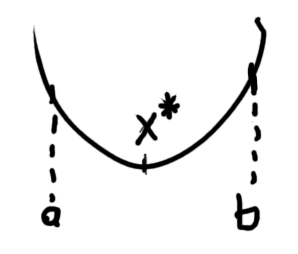
\includegraphics[width=3cm]{fig/unconstrained/6_11.png} For an $x \in [a, b]$ we have $f(x) \geq f(x*)$

\begin{minipage}[t]{.5\textwidth}
  \textbf{From $a$ to $x^*$}\\
  \\
  We have $x < x^*$ and $f(x) - f(x^*) \geq 0$ thus
  \[
  	\frac{f(x) - f(x^*)}{x - x^*} \leq 0
  \]
\end{minipage}
\hspace{0.025\textwidth}\vline\hspace{0.025\textwidth}
\begin{minipage}[t]{.5\textwidth}
  \textbf{From $b$ to $x^*$}\\
  \\
  We have $x > x^*$ and $f(x) - f(x^*) \geq 0$ thus
  \[
  	\frac{f(x) - f(x^*)}{x - x^*} \geq 0
  \]
\end{minipage}

Going back to the definition of a limit we have

\begin{minipage}[t]{.5\textwidth}
  \[
  	\lim_{d\to\infty} \frac{f(x^* + d) - f(x)}{d} \leq 0
  \]
\end{minipage}
\hspace{0.025\textwidth}\vline\hspace{0.025\textwidth}
\begin{minipage}[t]{.5\textwidth}
  \[
  	\lim_{d\to\infty} \frac{f(x^* + d) - f(x)}{d} \geq 0
  \]
\end{minipage}
\\
\\

\hspace{0.5in} \textit{N2 if $x^*$ is a local minimum and $f \in \mathcal{C}^2$, then $\nabla f(x^*) = 0$ and $\nabla^2 f(x^*) = 0$}

If $f \in \mathcal{C}^2$ then $f \in \mathcal{C}^1$ is also true, thus the previous results apply.

\incomplete

\subsection{Exercise 10/71 - Unconstrained optimization with a quadratic objective}
In S2, show that $s^*$ is in fact a \textit{global} minimum!

\textbf{Answer}

\hspace{0.5in} S2 if $Hs^* = -g$ and $H \prec 0$ then $s^*$ is a local minimum

Since $q(s)$ is a quadratic, a local minimum $s*$ of $q$ is automatically a global minimum.

\subsection{Exercise 46/71 - Conjugate gradient \textcolor{green}{???}}
Show that conjugate vectors are necessarily linearly independent.

\answer

Proof by contradiction. If $p_i$ is linearly dependant to a $p_j$ then we have
\[
	a_0 p_0 + a_1 p_1 + \ldots + a_n p_n = 0 \hspace{1cm} n \in \mathbb{Z^*}
\]

Where all $a_n$ are non-zero. Multiply by A
\[
	a_i p_i^T A= 0
\] 
Take the scalar product with $p_i$
\[
	a_i p_i^T A p_i = 0
\]
We know that $A \succ 0$ which means that $p_i^T A p_i > 0$ thus $a_i = 0$ which is contradictory to a linearly dependant system.

\subsection{Exercise 47/71 - Conjugate gradient}

Explain geometrically why $r_{k+1} \perp r_k$ i.e. $r_{k+1}^T r_k = 0$

\answer

When doing a linesearch we stop at a point where the direction is minimal. This also means we are tangent to the contour line (level curve), thus the next direction is orthogonal to the current one.

\begin{center}
	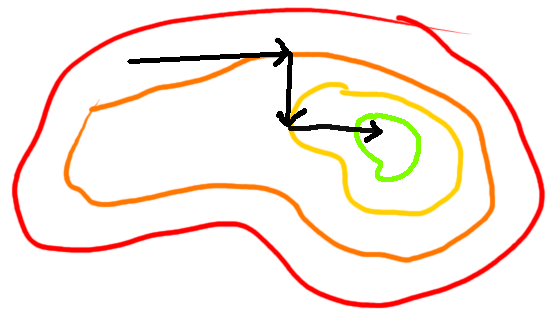
\includegraphics[width=5cm]{fig/unconstrained/47_71.png}
\end{center}


\subsection{Exercise 47/71 - Conjugate gradient}

Find a recurrence to update $q(x_k)$ in the conjugate gradient algorithm.

\answer

Should be something like 
\[
	q(x_{k+1}) = q(x_k) + \nabla q(x_k) \alpha_k A p_k
\]
So the current value of $q$ plus the change in $q$ and how much of that change.

\incomplete

\subsection{Exercice 48/71 - Conjugate gradient}
Prove $A \succ 0$ if and only if $p_k^T A p_k > 0$ for all $k = 0,\ \ldots,\ n-1$

\answer

We know that $A \succ 0$ if all the eigen values $\lambda$ of $A$ are positive and
\[
	A \textbf{v} = \lambda \textbf{v}
\]
so we can rewrite the expression as
\begin{align*}
	p_k^T A p_k = p_k^T \lambda p_k &> 0 \\
	\lambda p_k^T p_k &> 0 \\
	\lambda \| p_k \|^2 &> 0 
\end{align*}
Since $\| p_k \|^2$ must be positive then $\lambda$ must also be positive. Therefore $A \succ 0$.












\pagebreak
\section{Modeling problems}

\subsection{Problem 1}
\begin{minipage}{0.45\textwidth}
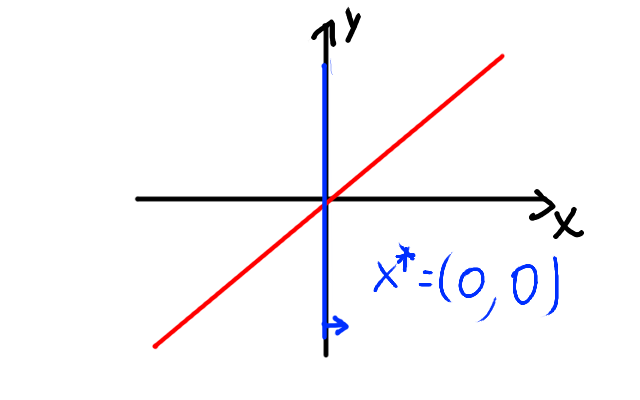
\includegraphics[width=\textwidth]{fig/model/1a.png}
1. a)
\end{minipage}
\hfill
\begin{minipage}{0.45\textwidth}
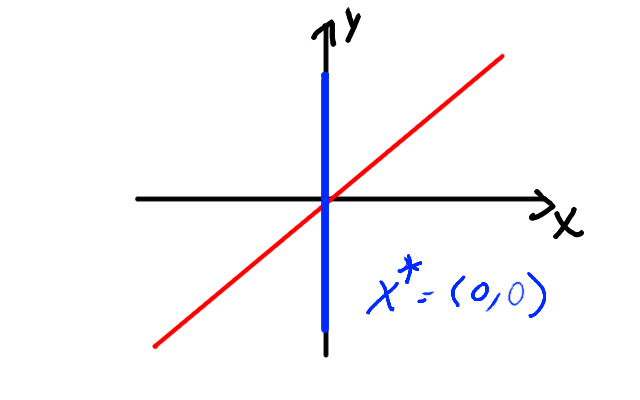
\includegraphics[width=\textwidth]{fig/model/1b.png}
1. b)
\end{minipage}

\begin{minipage}{0.45\textwidth}
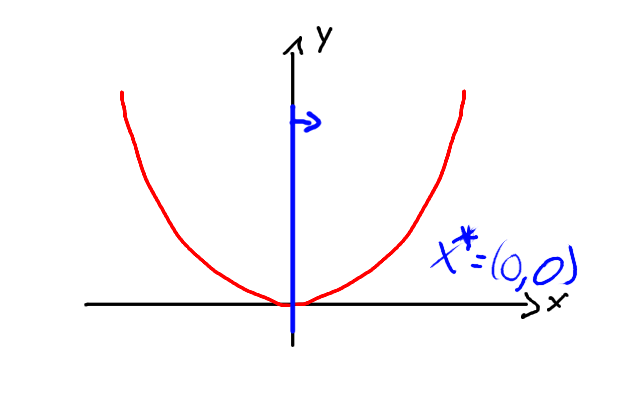
\includegraphics[width=\textwidth]{fig/model/1c.png}
1. c)
\end{minipage}
\hfill
\begin{minipage}{0.45\textwidth}
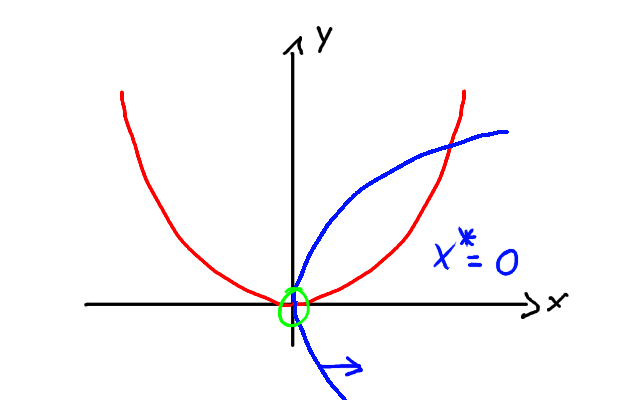
\includegraphics[width=\textwidth]{fig/model/1d.png}
1. d)
\end{minipage}

\begin{minipage}{0.45\textwidth}
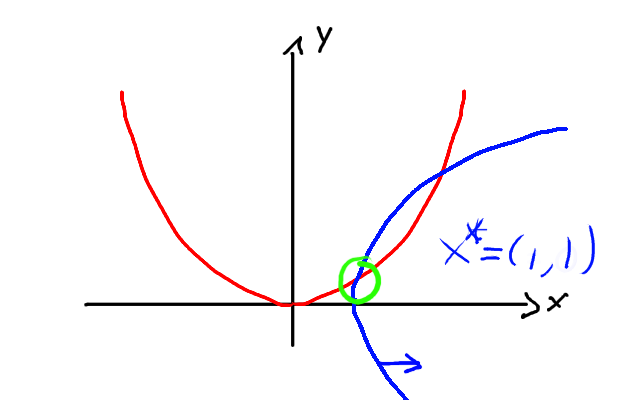
\includegraphics[width=\textwidth]{fig/model/1e.png}
1. e)
\end{minipage}

\pagebreak

\subsection{Problem 2}
\begin{figure}[h]
	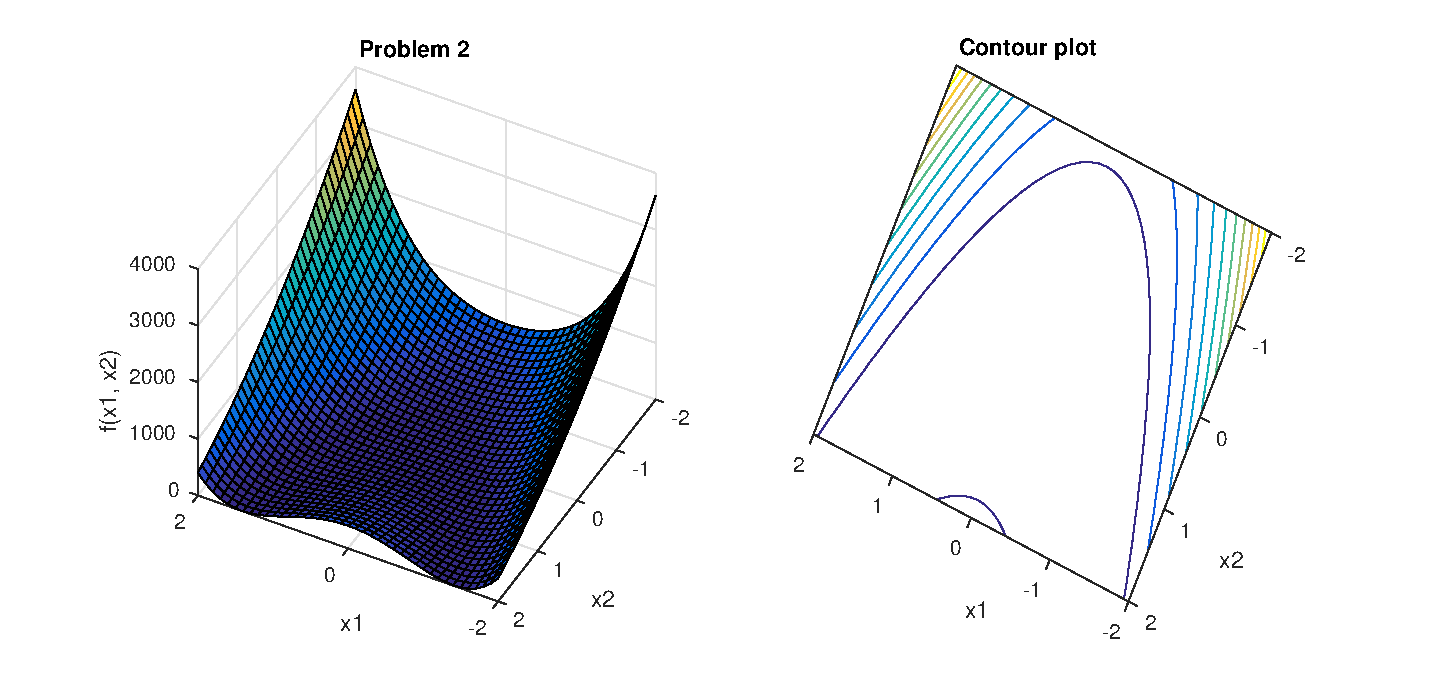
\includegraphics[width=\textwidth]{fig/model/problem2}
\end{figure}

\textbf{2.a)} We see that the two terms containing variables are square therefore the minimum is probably $0$. We can get this result with $x^* = (1,1)$ it is unique because of it is the only root of $100(x_2 - x_1^2)^2 + (1-x_1)^2$.

\textbf{2.b)} 

\lstset{ 
    language=AMPL, % choose the language of the code
    basicstyle=\fontfamily{ttfamily}\selectfont\footnotesize\color{black},
    keywordstyle=\color{blue}\bfseries, % style for keywords
    numbers=left, % where to put the line-numbers
    backgroundcolor=\color{white},
    showspaces=false, % show spaces adding particular underscores
    showstringspaces=false, % underline spaces within strings
    showtabs=false, % show tabs within strings adding particular underscores
    frame=single, % adds a frame around the code
    tabsize=4,
    rulesepcolor=\color{gray},
    rulecolor=\color{black},
    captionpos=b, % sets the caption-position to bottom
    breaklines=true, % sets automatic line breaking
    breakatwhitespace=false, 
}
\begin{lstlisting}
model;

var x1;
var x2;

minimize function:
	100 * (x2 - x1^2)^2 + (1 - x1)^2
\end{lstlisting}

Output:

\begin{lstlisting}[language=]
ampl: model modeling_pb2.mod;
ampl: solve;
MINOS 5.51: optimal solution found.
17 iterations, objective 9.247040366e-19
Nonlin evals: obj = 47, grad = 46.
ampl: display x1, x2;
x1 = 1
x2 = 1
\end{lstlisting}

Which confirms answer in \textbf{2.a)}.

\textbf{2.c)}  Add an equality constraint which changes the solution.
\begin{lstlisting}
model;

var x1;
var x2;

minimize function:
	100 * (x2 - x1^2)^2 + (1 - x1)^2;
	
subject to changeSolutionEqualityConstraint:
	x1 = 2;
\end{lstlisting}

Output:

\begin{lstlisting}[language=]
ampl: model modeling_pb2.mod;
ampl: solve;
MINOS 5.51: optimal solution found.
2 iterations, objective 1
Nonlin evals: obj = 6, grad = 5.
ampl: display x1, x2;
x1 = 2
x2 = 4
\end{lstlisting}

\textbf{2.d)}  Add an equality constraint which \textbf{does not} change the solution.
\begin{lstlisting}
model;

var x1;
var x2;

minimize function:
	100 * (x2 - x1^2)^2 + (1 - x1)^2;
	
subject to dontChangeSolutionEqualityConstraint:
	x1 = 1;
\end{lstlisting}

Output:

\begin{lstlisting}[language=]
ampl: model modeling_pb2.mod;
ampl: solve;
MINOS 5.51: optimal solution found.
2 iterations, objective 0
Nonlin evals: obj = 6, grad = 5.
ampl: display x1, x2;
x1 = 1
x2 = 1
\end{lstlisting}


\textbf{2.e)}  Add an inequality constraint which changes the solution.
\begin{lstlisting}
model;

var x1;
var x2;

minimize function:
	100 * (x2 - x1^2)^2 + (1 - x1)^2;
	
subject to changeSolutionInequalityConstraint:
	x1 >= 2;
\end{lstlisting}

Output:

\begin{lstlisting}[language=]
ampl: model modeling_pb2.mod;
ampl: solve;
MINOS 5.51: optimal solution found.
2 iterations, objective 1
Nonlin evals: obj = 6, grad = 5.
ampl: display x1, x2;
x1 = 2
x2 = 4
\end{lstlisting}

\textbf{2.f)}  Add an inequality constraint which \textbf{does not} changes the solution.
\begin{lstlisting}
model;

var x1;
var x2;

minimize function:
	100 * (x2 - x1^2)^2 + (1 - x1)^2;
	
subject to dontChangeSolutionInequalityConstraint:
	x1 <= 2;
\end{lstlisting}

Output:

\begin{lstlisting}[language=]
ampl: model modeling_pb2.mod;
ampl: solve;
MINOS 5.51: optimal solution found.
17 iterations, objective 9.247040366e-19
Nonlin evals: obj = 47, grad = 46.
ampl: display x1, x2;
x1 = 1
x2 = 1
\end{lstlisting}

\subsection{Problem 3}

Model:

\begin{lstlisting}
model;

var x1;
var x2;

minimize function:
	(x1 - 2)^2 + (x2 -1)^2;
	
subject to zeroConstraint:
	x1^2 - x2 <= 0;
	
subject to twoConstraint:
	x1 + x2 <= 2;
\end{lstlisting}

Output:

\begin{lstlisting}[language=]
ampl: model modeling_pb3.mod;
ampl: solve;
MINOS 5.51: optimal solution found.
12 iterations, objective 1
Nonlin evals: obj = 33, grad = 32, constrs = 33, Jac = 32.
ampl: display x1, x2;
x1 = 1
x2 = 1
\end{lstlisting}

\subsection{Problem 4}

\textbf{4.a)}

\begin{align*}
P_3(x) &= \frac{f^{(0)}(x_0)}{0!} + \frac{f^{(1)}(x_0)}{1!}(x - x_0) + \frac{f^{(2)}(x_0)}{2!}(x - x_0)^2 + \frac{f^{(3)}(x_0)}{3!}(x - x_0)^3\\
&= \cos(1) + \frac{-\sin(1)}{1} (x-1) + \frac{-\cos(1)}{2} (x - 1)^2 + \frac{\sin(1)}{6}(x-1)^3\\
\text{For x = 1.1 we have}\\
P_3(1.1) &= \cos(1) + (-0.0841) + (-0.0027) + (0.0001)\\
&= 0.4536
\end{align*}

\textbf{4.b)}

\begin{align*}
f(x) &= \cos(x) \\
f'(x) &= \sin(\frac{1}{x}) \frac{1}{x^2}\\
f''(x) &= \Big( \sin(\frac{1}{x}) \Big)' \frac{1}{x^2} + \sin(\frac{1}{x}) \Big( \frac{1}{x^2}\Big)'\\
&= \cos(\frac{1}{x})\frac{-1}{x^2}\frac{1}{x^2} + \sin(\frac{1}{x}) \frac{-2}{x^3}\\
&= -\frac{\cos(\frac{1}{x}) + 2x\sin(\frac{1}{x})}{x^4}
\end{align*}

Thus the 2nd order Taylor expansion with $x_0 = 1$ is
\begin{align*}
P_2(x) = \cos(1) + \sin(1)(x-1) - \Big( \frac{\cos(1)+2\sin(1)}{2} \Big)(x - 1)^2
\end{align*}

And for $x = 1.1$ we have
\begin{align*}
P_2(1.1) &= \cos(1) + \sin(1)(1.1-1) - \Big( \frac{\cos(1)+2\sin(1)}{2} \Big)(1.1 - 1)^2\\
&= 0.5403 + 0.0841 - 0.0111\\
&= 0.6133
\end{align*}

\pagebreak

\textbf{4.c)}

\begin{align*}
f_{x_1} &= -200(x_1^2 + 2x_1 - x_2) + 2(x_1 -1)  \\
f_{x_2} &= 200(x_2 - x_1^2)\\
f_{x_1 x_1} &= -200 (2x_1 + 2) + 2\\
f_{x_1 x_2} &= -200(-1) = 200\\
f_{x_2 x_1} &=  200(1-2x_1)\\
f_{x_2 x_2} &= 200
\end{align*}

Thus the Taylor expansion in matrix form is

\[
f(x,y) = f(0,0) +
	\begin{bmatrix}
	x \\
	y
	\end{bmatrix}^T
	\begin{bmatrix}
		-200(x_1^2 + 2x_1 - x_2) + 2(x_1 -1) \\
		200(x_2 - x_1^2)
	\end{bmatrix}
+ \frac{1}{2!}
	\begin{bmatrix}
	x \\
	y
	\end{bmatrix}^T
	\begin{bmatrix}
    	-200 (2x_1 + 2) + 2 & 200\\
    	200(1-2x_1) & 200
	\end{bmatrix}	
	\begin{bmatrix}
	x \\
	y
	\end{bmatrix}
\]

\textbf{4.d)}

Around the point $(x, y) = (a, b)$ we have
\begin{align*}
f(x, y) &= f(a, b) + 
\Bigg( 
	\begin{bmatrix}
    	x \\
    	y
	\end{bmatrix}
	-
	\begin{bmatrix}
    	a \\
    	b
	\end{bmatrix}
\Bigg)^T
	\begin{bmatrix}
    	f_x(a,b) \\
    	f_y(a,b)
	\end{bmatrix}
+
\frac{1}{2!}
\Bigg( 
	\begin{bmatrix}
    	x \\
    	y
	\end{bmatrix}
	-
	\begin{bmatrix}
    	a \\
    	b
	\end{bmatrix}
\Bigg)^T
	\begin{bmatrix}
    	f_{xx}(a,b) & f_{xy}(a,b)\\
    	f_{yx}(a,b) & f_{yy}(a,b)
	\end{bmatrix}
\Bigg( 
	\begin{bmatrix}
    	x \\
    	y
	\end{bmatrix}
	-
	\begin{bmatrix}
    	a \\
    	b
	\end{bmatrix}
\Bigg)
\end{align*}

\subsection{Problem 5}

In the folowing problems we denote $x = \begin{bmatrix}x_1 & x_2 & \ldots x_n \end{bmatrix}$

\textbf{Function $f_1$}

\[
f_1(x) = c^T x =
\begin{bmatrix}
	c_1 \\ c_2 \\ \vdots \\ c_n
\end{bmatrix}
\begin{bmatrix}
	x_1 & x_2 & \ldots & x_n
\end{bmatrix}
\]

The gradient is then given by

\[
\nabla f_1(x) = 
\begin{bmatrix}
	c_1 \frac{\partial f}{x_1} \\ 
	c_2 \frac{\partial f}{x_2} \\ 
	\vdots \\ 
	c_n \frac{\partial f}{x_n}
\end{bmatrix}
=
\begin{bmatrix}
	c_1 \\ 
	c_2\\ 
	\vdots \\ 
	c_n 
\end{bmatrix}
\]

And the Hessian is given by 
\[
\textbf{H} = 
\begin{bmatrix}
0 & \ldots & 0 \\
\vdots & \ddots & \vdots \\
0 & \ldots & 0
\end{bmatrix}
\]

since the gradient was all constants.

\textbf{Function $f_2$}


\[
f_2(x) = \frac{1}{2} x^T H x
\]














\end{document}


